% ------------------------------------------------------------------------
% ------------------------------------------------------------------------
% ------------------------------------------------------------------------
%                                Capítulo 3
% ------------------------------------------------------------------------
% ------------------------------------------------------------------------
% ------------------------------------------------------------------------
\chapter{BÚSQUEDA DE LOS OXINITRUROS RP MÁS ESTABLES}\label{Cap. 2}

Este capítulo presenta un análisis estructural de los oxinitruros \textsc{rp} $Sr_{2}(Ta,Nb)O_{4-x}N_{x}$ y la búsqueda de los ordenamientos aniónicos más estables. Inicia con una breve descripción de óxidos de perovskitas \textsc{rp}, luego describe la substitución aniónica parcial $x=0.5$ de $O^{2-}$ por $N^{3-}$, y la substitución parcial $x=1$ de $O^{2-}$ por $N^{3-}$. Las substituciones aniónicas se realizan con el programa \textsc{sod}\cite{Grau-Crespo2007}, el cual es un paquete de herramientas para modelado computacional de sistemas periódicos con desorden substitucional de sitio. Un sistema desordenado es modelado como una copia de la celda, en donde combinaciones diferentes de desorden son puestas en los sitios cristalográficos. La celda diferente a la celda original es llamada \textit{'configuración'}. El proceso de identificar la simetría de cada configuración se realiza con las operaciones de simetría del grupo cristalográfico al que corresponde. Posteriormente, se identifican las configuraciones simétricamente equivalentes, y solo las configuraciones con simetría única son tomadas en cuenta. Una vez se identifican las configuraciones únicas, el código \textsc{sod} muestra las configuraciones únicas, y su degenerancia, es decir las configuraciones equivalentes \cite{Grau-Crespo2007}.

%sustituye los átomos y calcula las ocupaciones de sitio dando un numero de configuraciones resultantes. Mediante la simetría cristalina de la red, el programa reduce el número de configuraciones, identifica las configuraciones inequivalentes con el grupo de simetría espacial, es decir, calcula la degenerancia de las configuraciones.

\begin{figure}[H]
    \centering
    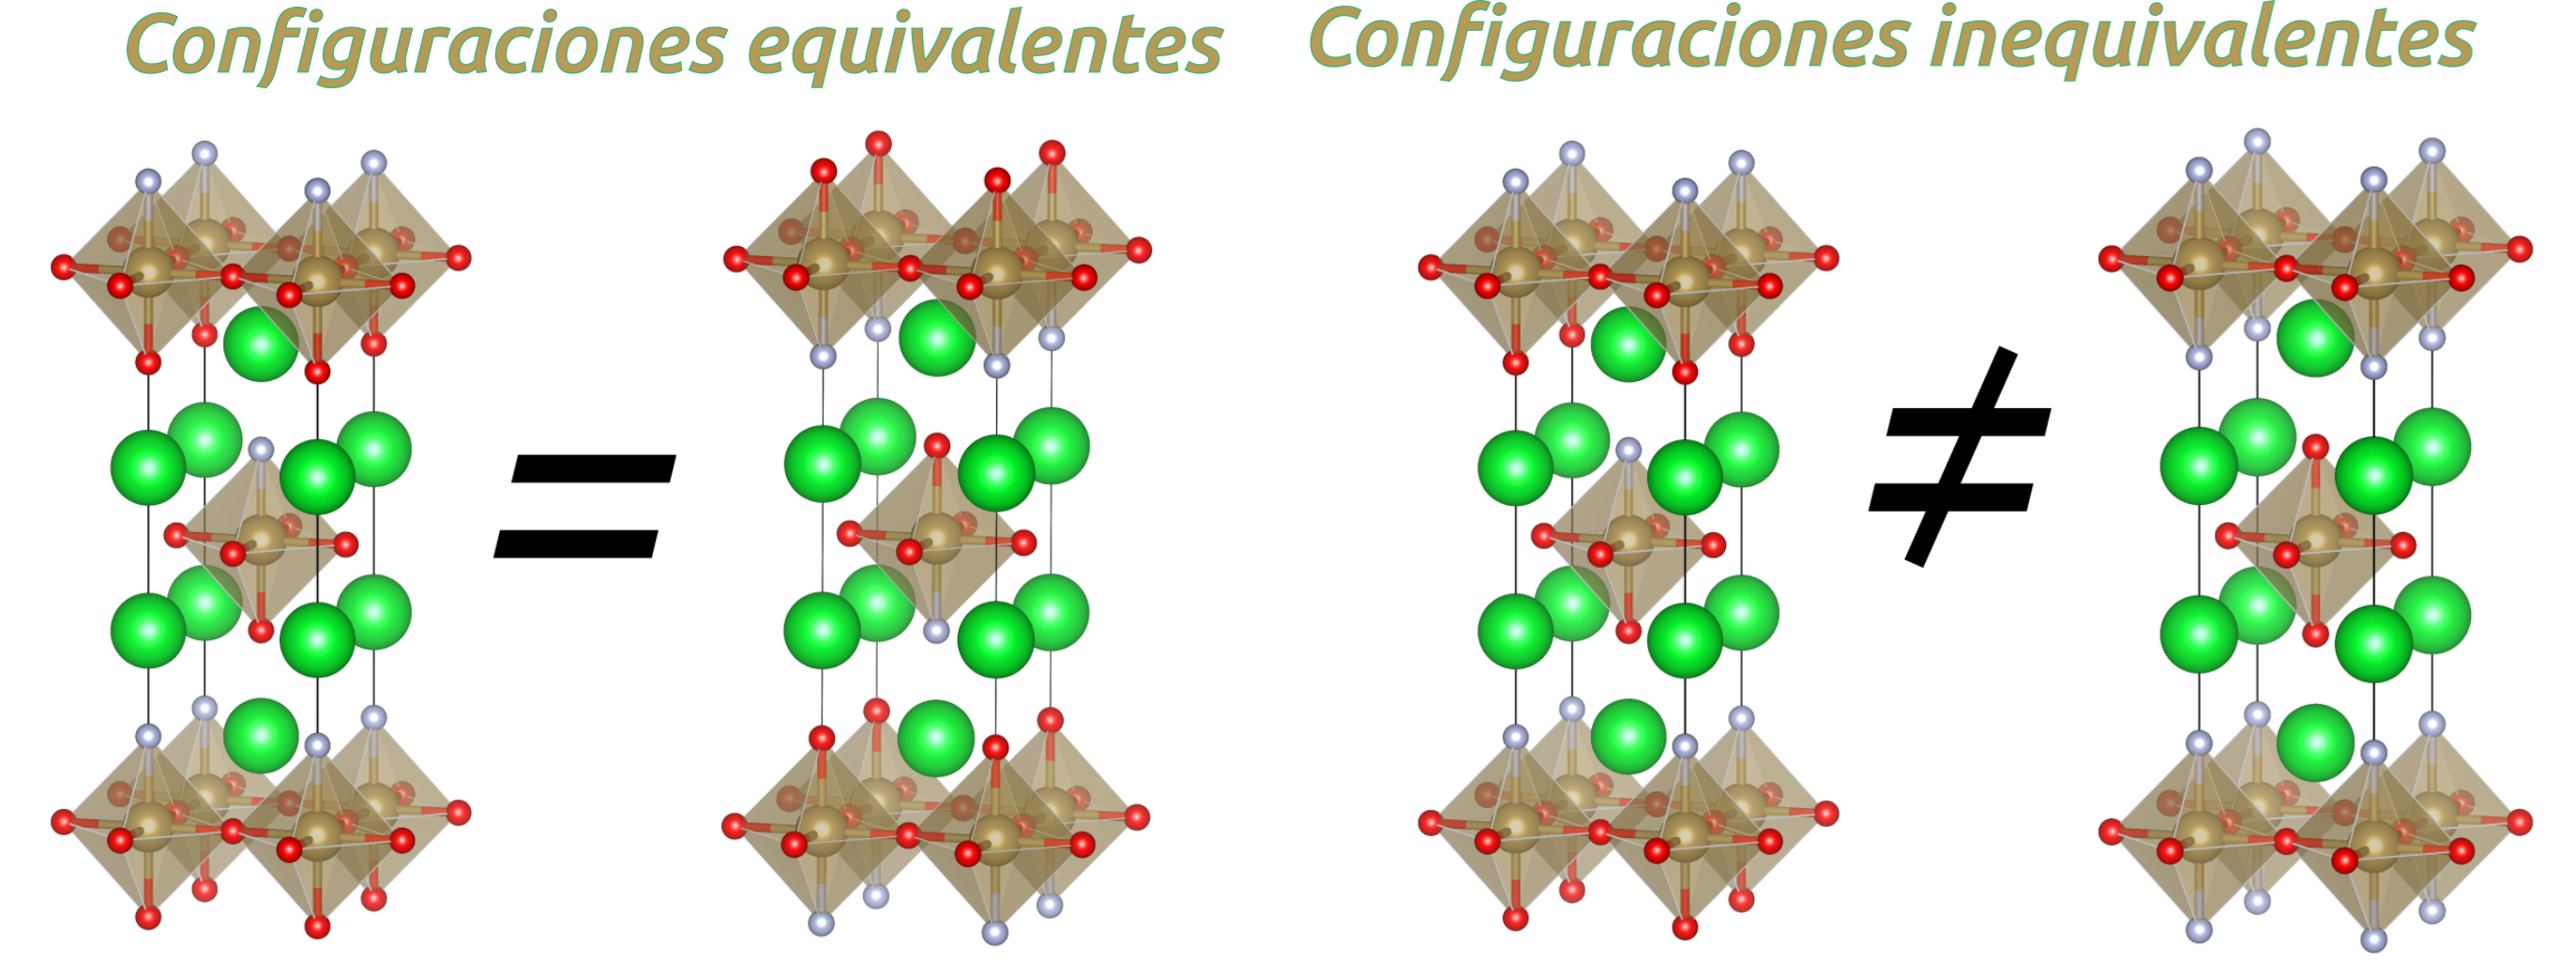
\includegraphics[width=0.9\textwidth]{Figs/config.png}
    \caption{Comparación de configuraciones equivalentes y configuraciones inequivalentes.}
    \label{Fig. config}
\end{figure}

El criterio de equivalencia entre dos configuraciones se basa en el concepto de las transformaciones isométricas, que son operaciones geométricas como traslaciones, rotaciones y reflexiones, para mantener constantes todas las distancias y ángulos dentro del objeto transformado. En la figura \ref{Fig. config} se aprecia que las configuraciones equivalentes son una misma configuración debido a que mediante una trasformación se puede verificar que una configuración es igual a la configuración sin transformar. En cambio, las configuraciones inequivalentes no tienen una transformación para obtener una configuración equivalente. El hecho de que dos configuraciones tengan el mismo grupo espacial no implica que tendrán la misma energía \cite{Grau-Crespo2007}. \textcolor{red}{??? si son el mismo grupo y la misma estequimetria, como cambia la energia?}

Finalizando con el capítulo, se presenta un análisis de la energía estructural de cada configuración. Además, con ayuda del programa \href{https://uspex-team.org/online_utilities/poscar2cif/}{\textsc{poscar2cif}}\cite{urlposcar2cif} se obtuvo el grupo espacial cristalográfico de cada configuración.

\section{SUBSTITUCIÓN ANIÓNICA EN LA ESTRUCTURA RUDDLESDEN-POPPER\\ Sr$_{2}$(Ta,Nb)O$_{4-x}$N$_{x}$(x=0.5 Y x=1.0)}
% ------------------------------------------------------------------------
La fase Ruddlesden-Popper (\textsc{rp}) en la que se enfoca este trabajo tiene como fórmula general $A_{n+1}B_{n}X_{3n+1}(n=1)$, donde $A$ y $B$ representan los cationes, y $X$ son los aniones de la estructura\cite{Beznosikov2000}. Los elementos que ocupan los sitios cristalográficos son los cationes estroncio $(Sr)$ para el sitio $A$, niobio ó tántalo $(Nb,Ta)$ para el sitio $B$, y oxigeno $(O)$ para el sitio $X$. Es decir, las dos estructuras cristalinas principales de la fase \textsc{rp} son $Sr_{2}TaO_{4}$ y $Sr_{2}NbO_{4}$ de la figura \ref{Fig. rp_nb-ta} obtenidas con el programa \textsc{vesta}\cite{Momma2011}. 
Estas estructuras cristalinas se representan con el grupo de simetría espacial cristalográfico $I4/mmm$ (139), tiene parámetros de celda $a$ = 4.02994 \r{A} y $c$ = 12.64448 \r{A},  $\alpha=\beta=\gamma=90^{\circ}$ y volumen de $205.35$ para $Sr_{2}TaO_{4}$, y $a$ = 4.04552 \r{A} y $c$ =12.74460 \r{A},  $\alpha=\beta=\gamma=90^{\circ}$ y volumen de $208.58$ para $Sr_{2}NbO_{4}$, según datos experimentales\cite{Clarke2002,Tobias2004,Diot1999CrystalN}.

\begin{figure}[H]
    \centering
    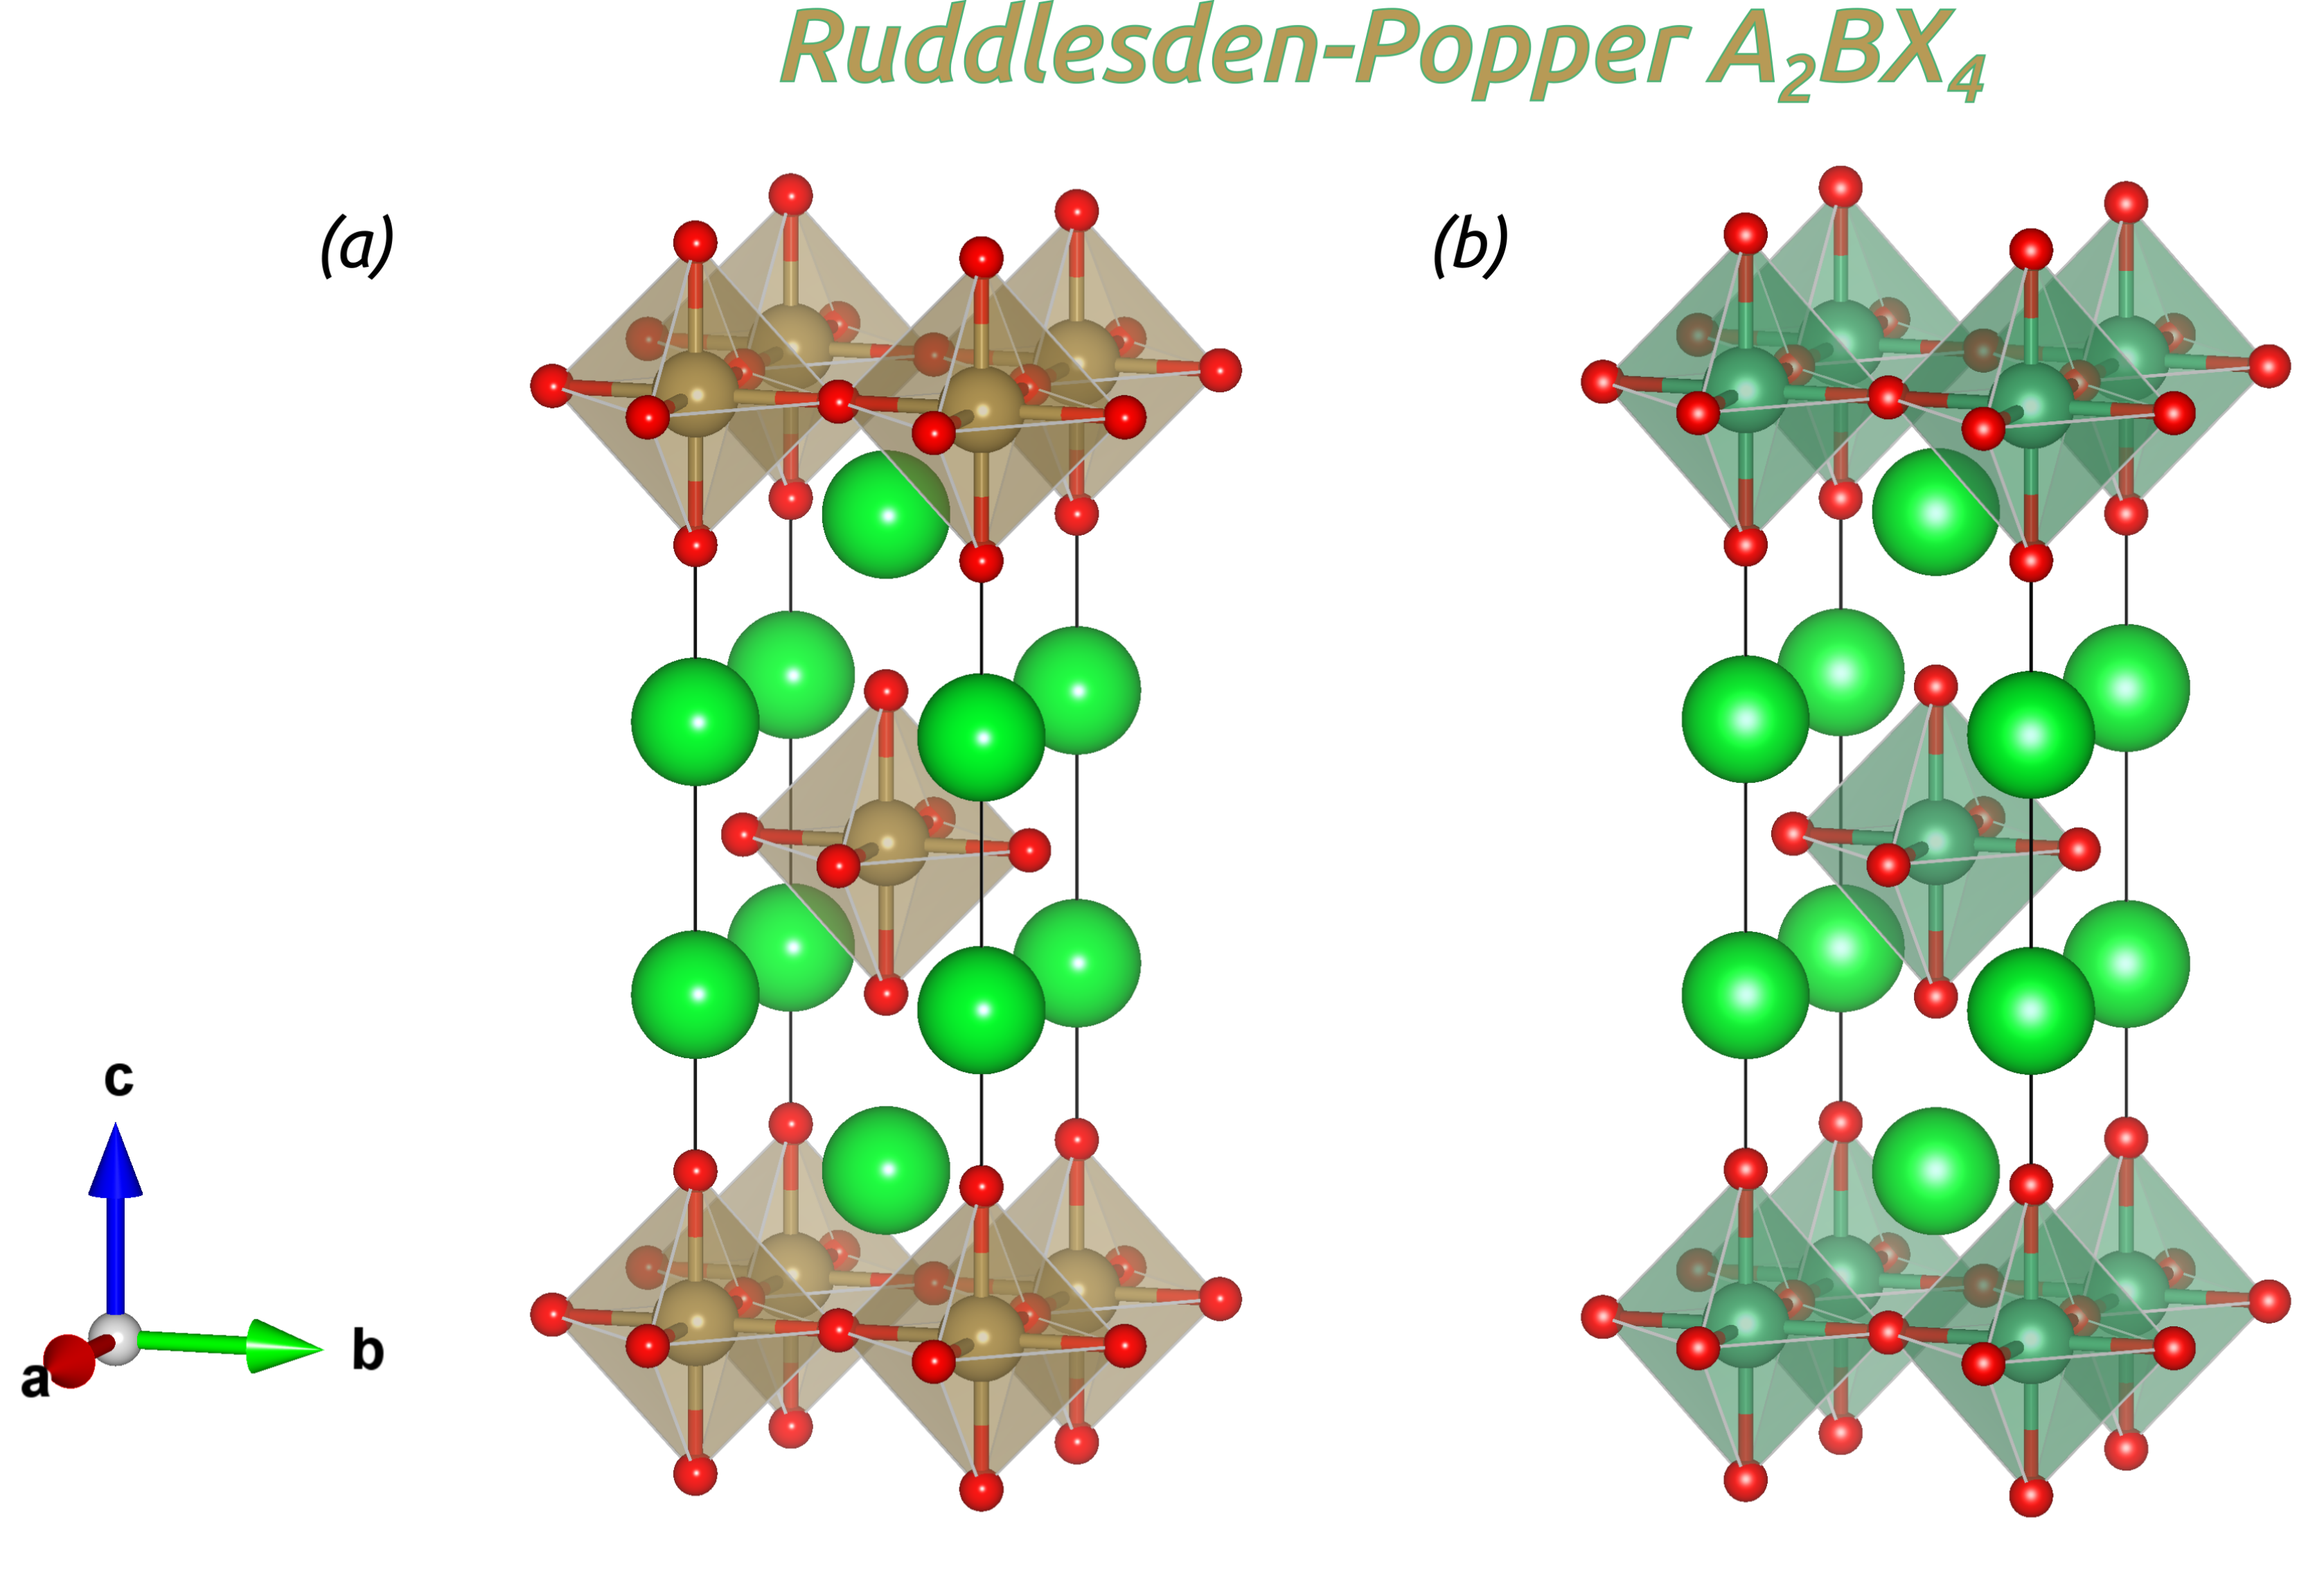
\includegraphics[width=0.6\textwidth]{Figs/rp_ta-nb.png}
    \caption{Estructuras cristalinas de la fase Ruddlesden-Popper: \textcolor{Sr}{$Sr_{2}$}\textcolor{Ta}{$Ta$}\textcolor{O}{$O_{4}$} y (b) \textcolor{Sr}{$Sr_{2}$}\textcolor{Nb}{$Nb$}\textcolor{O}{$O_{4}$}.}
    \label{Fig. rp_nb-ta}
\end{figure}

Modelar desorden en cristales es deseable debido a su estabilidad termodinámica y a propiedades sensibles al desorden.  El desorden en un cristal puede tomar varias formas: desorden dinámico \cite{Chick2009analysis}, desorden estático continuo y desorden estático discreto \cite{Muller2009structures}. Este ultimo contiene el tipo de 'desorden substitucional' \cite{Habgood2011model}, donde se substituye un anión por otro anión, lo cual hace el código \textsc{sod}\cite{Grau-Crespo2007}. Cuando se realizan substituciones isovalentes, como substituir aniones con igual oxidación como $O^{2-}$ por $S^{2-}$, trae consigo cambios sutiles a la estructura y sus propiedades. Sin embargo, la substitución de aniones aliovalentes, como $O^{2-}$ por $N^{3-}$, brindan cambios significativos en la estructura del material y sus propiedades electrónicas\cite{Roy2019}. Los oxinitruros \textsc{rp} con fórmula $Sr_{2}TaO_{3-x}N_{x}$ y $Sr_{2}NbO_{3-x}N_{x}$ preparados para substitución parcial del anión $O^{2-}$ por el anión $N^{3-}$ han recibido atención en recientes años debido a su potencial aplicación en dieléctricos, ferroeléctricos, fotocatálisis y materiales magneto-resistivos\cite{Fuertes2011}. La substitución de aniones en óxidos, sulfuros y otros materiales es comúnmente empleada para cambiar la estructura y sus propiedades dependiendo si la substitución es isovalente o aliovalente. 

\subsection{Substitución parcial x=0.5 en \textsc{rp}}

La fórmula de la fase oxinitrada \textsc{rp} con substitución parcial $x=0.5$ es: $Sr_{2}TaO_{3.5}N_{0.5}$ y  $Sr_{2}NbO_{3.5}N_{0.5}$. El nitrógeno $N^{3-}$ tiene la posibilidad de ocupar cualquier sitio cristalográfico del oxigeno $O^{2-}$ bajo la restricción de la simetría del grupo espacial $I4/mmm$ (SG. 139), esto conduce a la existencia de un numero finito de configuraciones posibles que pueden ser similares entre si debido a la simetría. El programa \textsc{sod} realiza las substituciones y define que configuraciones son independientes y que configuraciones son equivalentes a las independientes, aprovechando la simetría del cristal\cite{Grau-Crespo2007}.

\begin{figure}[H]
    \centering
    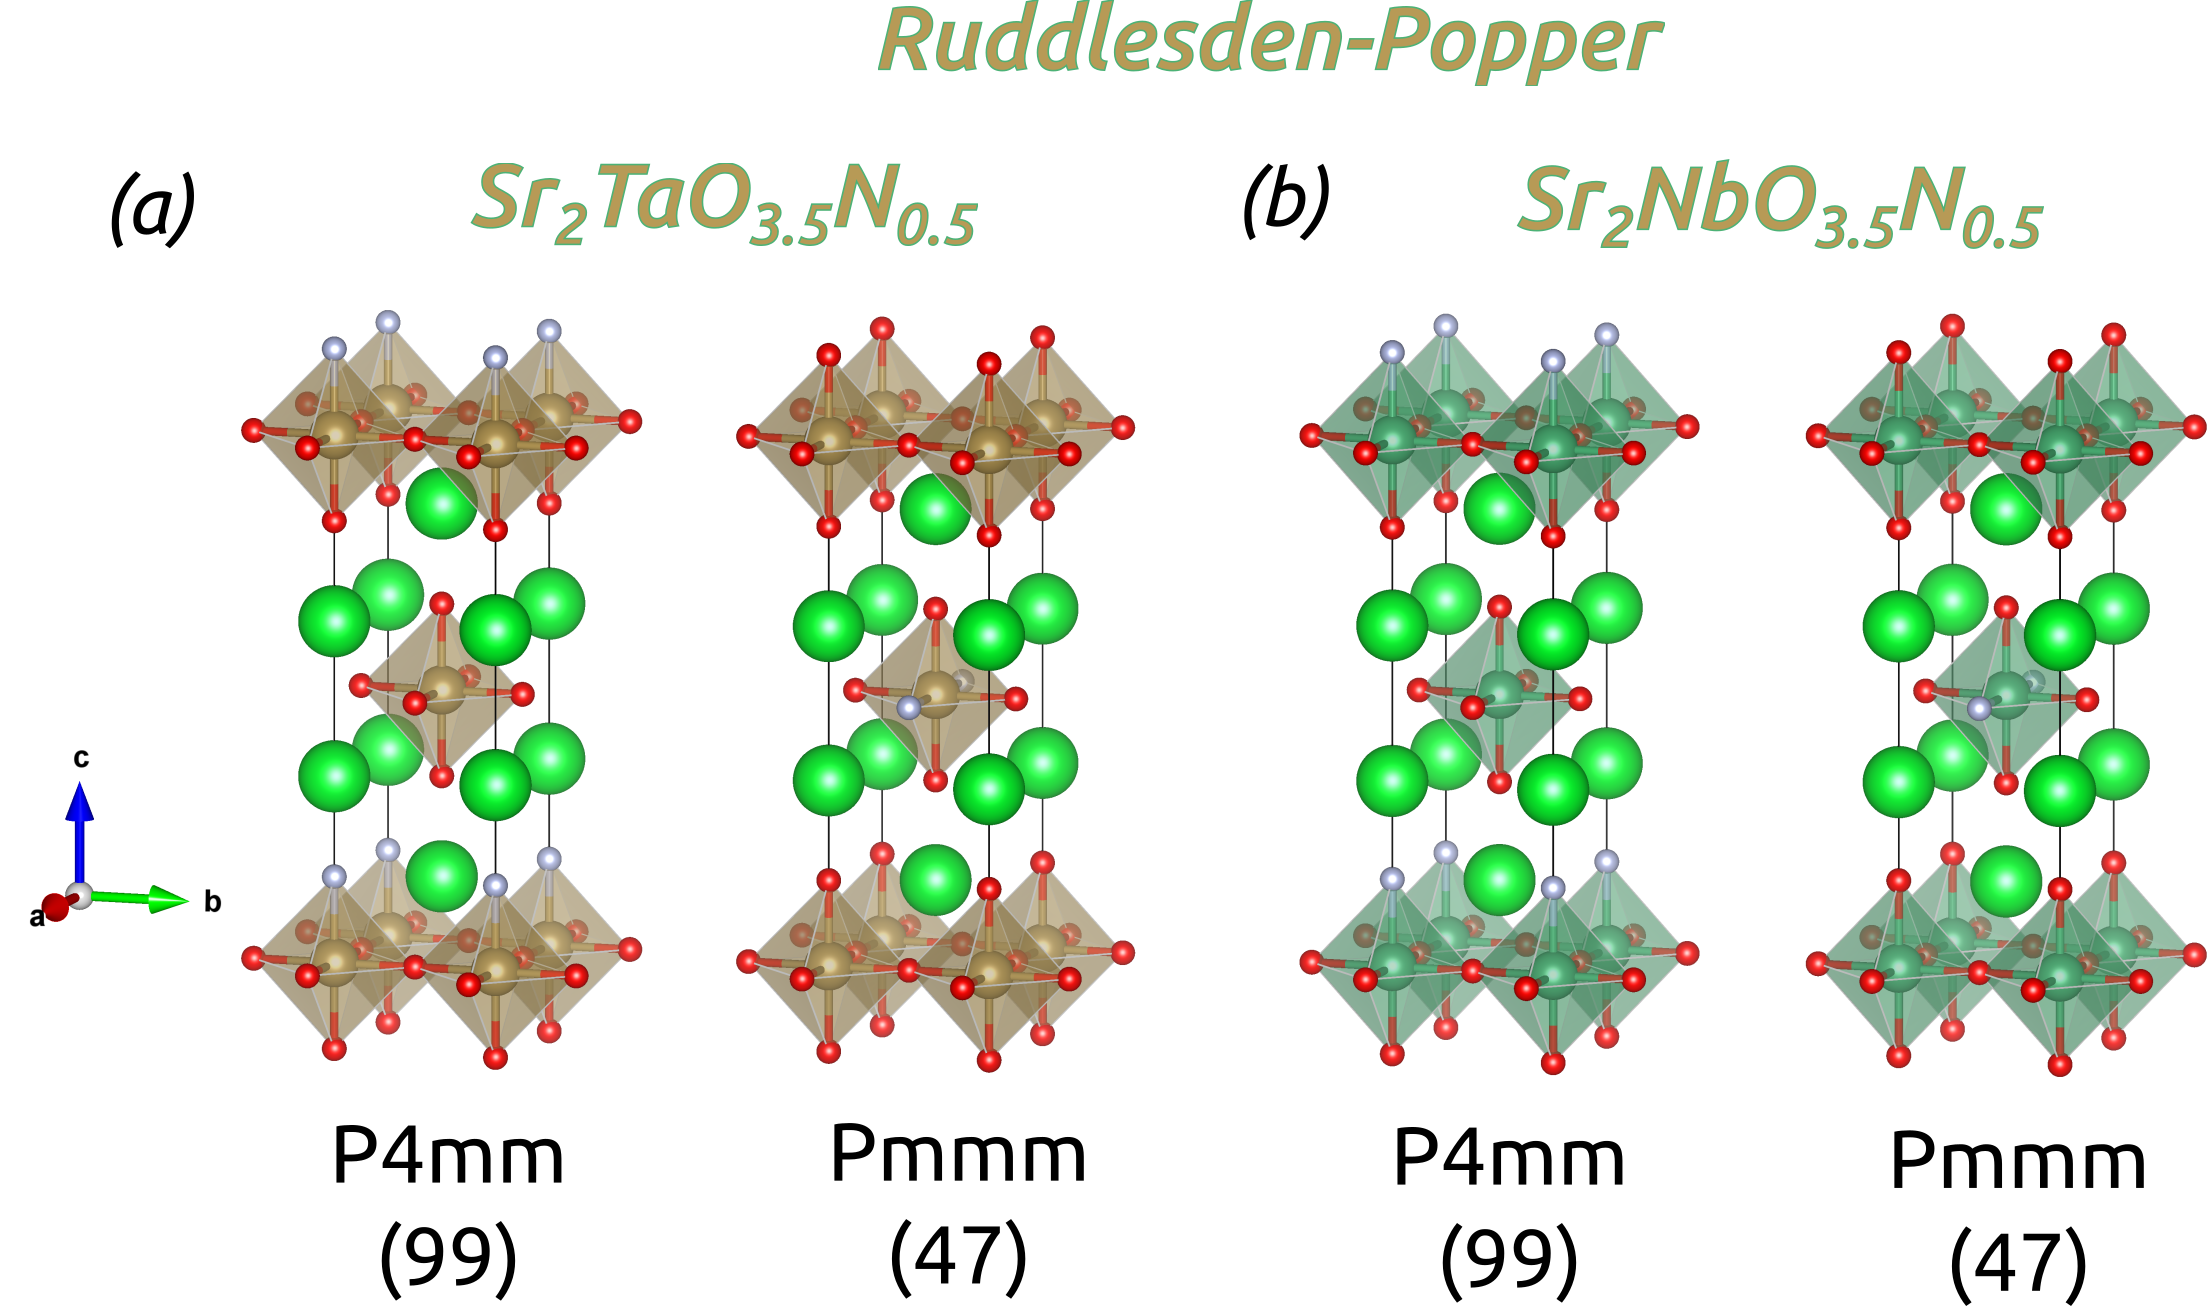
\includegraphics[width=0.7\textwidth]{Figs/rp_05.png}
    \caption{Estructuras cristalinas de la fase Ruddlesden-Popper después de substituir un oxigeno por un nitrógeno: (a) \textcolor{Sr}{$Sr_{2}$}\textcolor{Ta}{$Ta$}\textcolor{O}{$O_{3.5}$}\textcolor{N}{$N_{0.5}$} y (b) \textcolor{Sr}{$Sr_{2}$}\textcolor{Nb}{$Nb$}\textcolor{O}{$O_{3.5}$}\textcolor{N}{$N_{0.5}$}.}
    \label{Fig. rp_05}
\end{figure}

Al realizar la substitución parcial $x=0.5$ se obtienen $8$ configuraciones en total, pero solo $2$ son independientes. Este resultado es el mismo tanto para $Sr_{2}TaO_{3.5}N_{0.5}$ como para  $Sr_{2}NbO_{3.5}N_{0.5}$. Las dos configuraciones encontradas tienen grupo de simetría espacial cristalográfico diferente a la simetría inicial, esto depende del sitio que ocupen los nitrógenos en la estructura. La primera configuración de las figuras \ref{Fig. rp_05}(a) y \ref{Fig. rp_05}(b) con simetría espacial $P4mm$ (SG. 99) muestran que los nitrógeno ocupan los sitios superiores en los octaedros de las esquinas, pero el octaedro central de la celda unitaria no tiene ningún nitrógeno. 
La segunda configuración de las figuras \ref{Fig. rp_05}(a) y \ref{Fig. rp_05}(b) con simetría espacial $Pmmm$ (SG. 47) muestran una ocupación del nitrógeno tipo \emph{'trans'} en la dirección \emph{'a'} únicamente en el octaedro central, pero ninguna ocupación del nitrógeno en los octaedros de las esquinas. El poco contenido de nitrógeno muestra que no puede ocupar sitios en todos los octaedros, por esta razón las únicas dos configuraciones de esta sustitución muestran nitrógeno en capas intercaladas.

\subsection{Substitución parcial x=1.0 en \textsc{rp}}

La fórmula de la fase oxinitrada \textsc{rp} con substitución parcial $x=1.0$ es: $Sr_{2}TaO_{3}N$ y  $Sr_{2}NbO_{3}N$. En este caso, el numero de configuraciones obtenidas después de la sustitución son $28$ configuraciones en total, y solo $8$ independientes. En la figura \ref{Fig. rp_1} se muestran las $8$ configuraciones con diferente ordenamiento aniónico, tanto para \textsc{rp}-$Sr_{2}TaO_{3}N$  como para \textsc{rp}-$Sr_{2}NbO_{3}N$.

\begin{figure}[H]
    \centering
    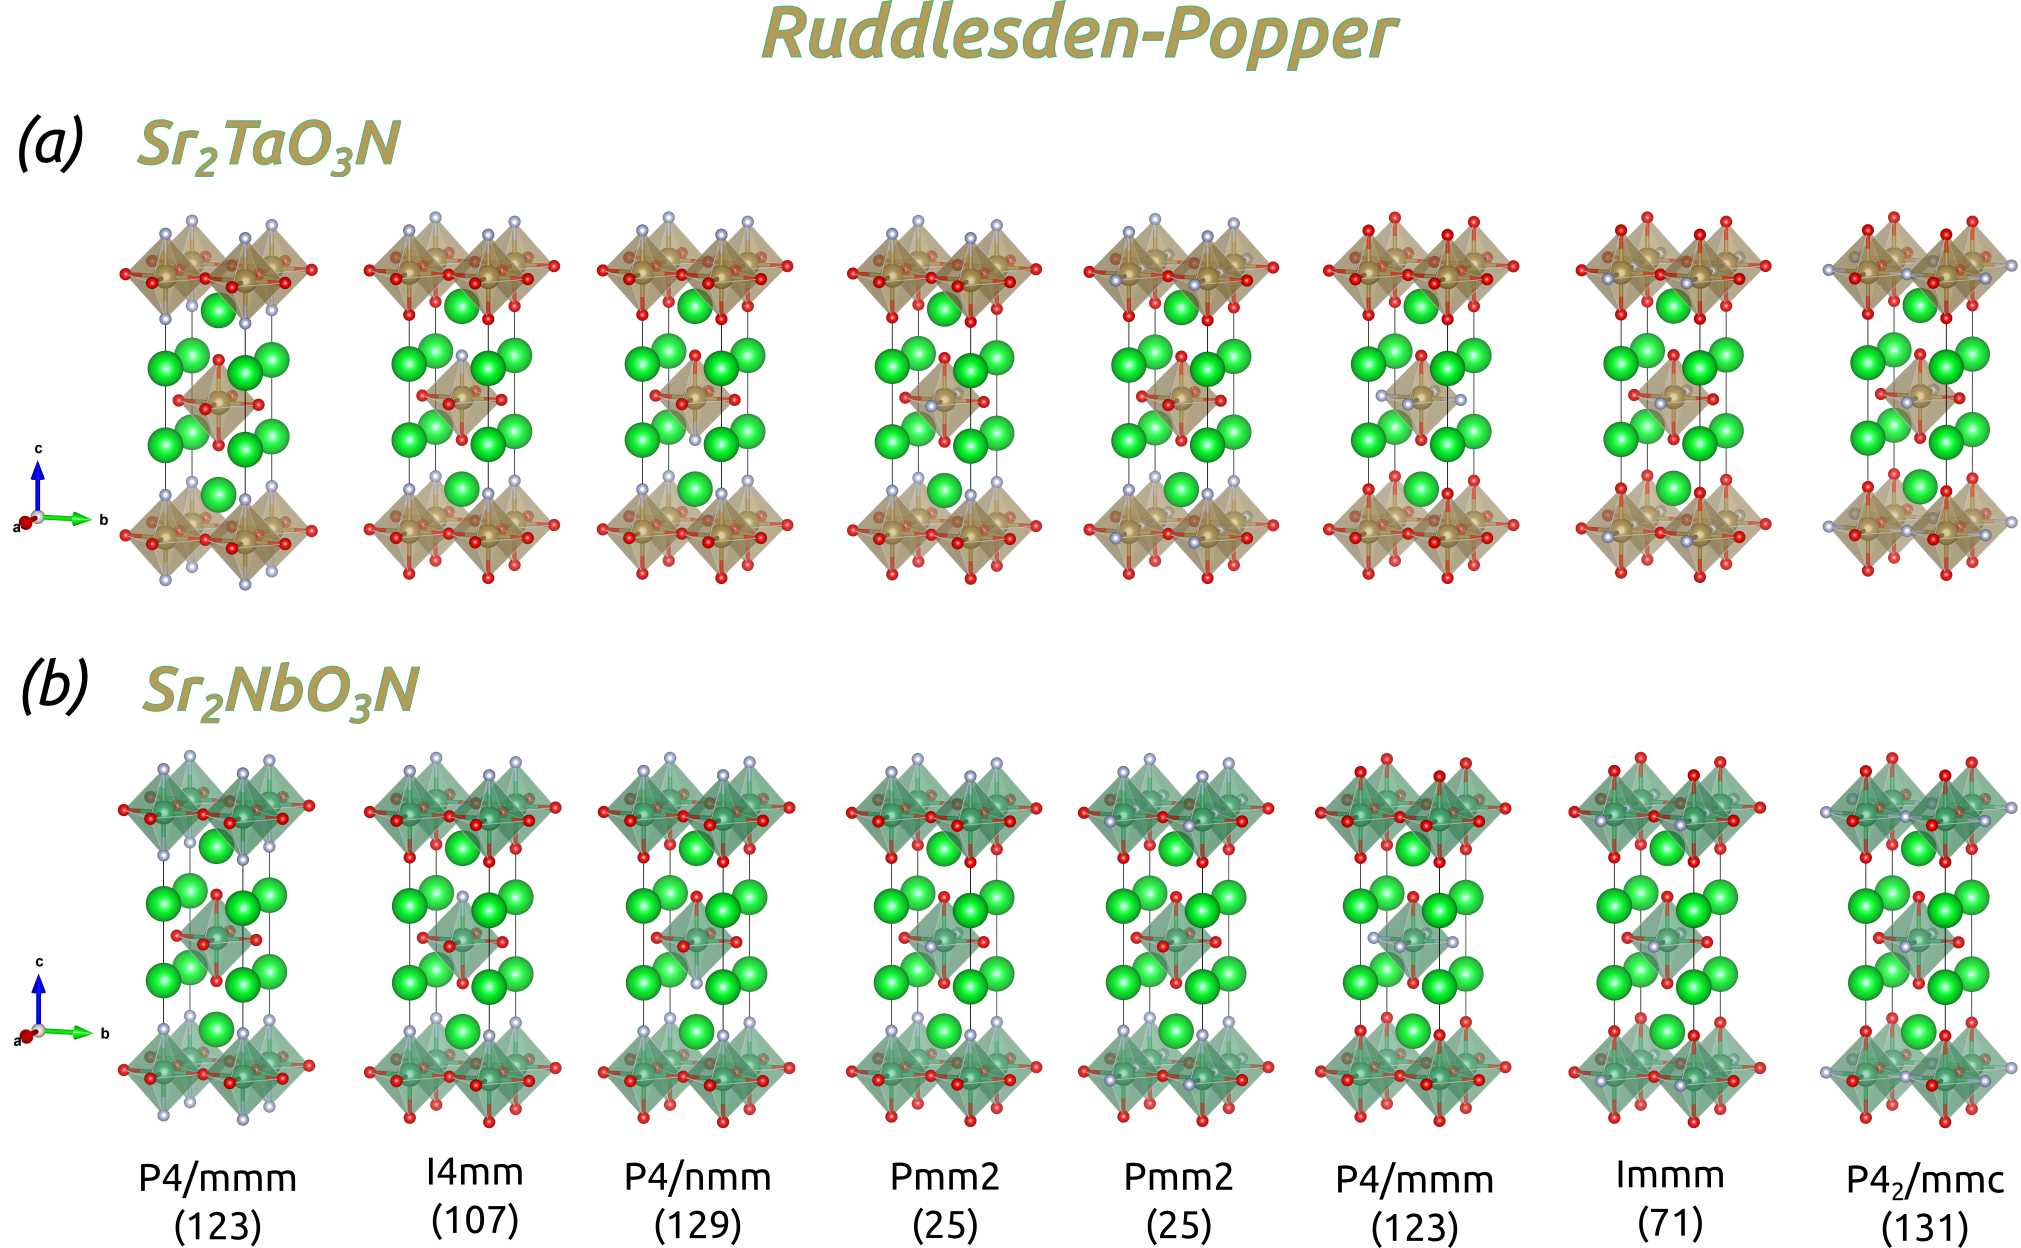
\includegraphics[width=\textwidth]{Figs/rp_1.png}
    \caption{Estructuras cristalinas de la fase Ruddlesden-Popper después de sustituir dos oxígenos por dos nitrógenos: (a) \textcolor{Sr}{$Sr_{2}$}\textcolor{Ta}{$Ta$}\textcolor{O}{$O_{3}$}\textcolor{N}{$N$} y (b) \textcolor{Sr}{$Sr_{2}$}\textcolor{Nb}{$Nb$}\textcolor{O}{$O_{3}$}\textcolor{N}{$N$}.}
    \label{Fig. rp_1}
\end{figure}

La primera configuración $P4/mmm$ (123) tiene el mismo grupo espacial que la configuración 6, pero diferente ordenamiento aniónico. La primera tiene ocupación de nitrógeno en los octaedros de las esquinas tipo \emph{trans} en la dirección \emph{'c'}, pero el octaedro central no tiene nitrógeno. Mientras que la configuración $6$ no tiene nitrógeno en los octaedro de las esquinas, pero el octaedro central evidencia una ocupación de oxigeno de tipo \emph{trans} en la dirección \emph{'c'}, es decir, los nitrógenos ocupan los sitios ecuatoriales del octaedro central.

Las configuraciones $I4mm$ (107) y $P4/nmm$ (129) tienen en común la ocupación del nitrógeno en el sitio superior del octaedro, pero con la diferencia de que el nitrógeno del octaedro central de la configuración 129 esta en el sitio inferior. Las dos configuraciones $Pmm2$ (25) tienen distintos ordenamientos aniónicos, el primero tiene $N$ en el sitio superior de los octaedros de las esquinas, mientras que el octaedro central tiene ordenamiento de $N$ tipo \emph{trans} en dirección \emph{'a'}; la segunda configuración no tiene $N$ en el octaedro central, pero tiene un ordenamiento particular tipo \emph{mer} en los octaedros de las esquinas. Las dos últimas configuraciones, $Immm$ (71) y $P4_{2}/mmc$ (131), tienen ordenamiento tipo \emph{trans} en todos sus octaedros, la configuración con grupo espacial $71$ tiene el ordenamiento de $N$ en dirección $a$, pero la configuración $131$ tienen el ordenamiento de $N$ en la dirección $b$ solo de los octaedros de las esquinas. El aumento de nitrógeno en la estructura hace que pueda ocupar mas sitios en el octaedro, haciendo que existan mas configuraciones que la substitución x=0.5.

% En todas las configuraciones presentadas no se observa ninguna relación entre el grupo espacial cristalográfico y el ordenamiento aniónico.\\

Al substituir los aniones en los sitios cristalográficas, el programa \textsc{sod} no tiene en cuenta si debe desplazar los sitios debido a las nuevas interacciones atómicas entre el metal de transición, $Ta/Nb$, y el nitrógeno, así que las estructuras deben pasar por un proceso de relajación para redefinir los sitios según las nuevas interacciones.
